\subsection{Completed spatial experiment and measured limitations}
\newcommand{\TeleBulkOrder}{5.89}
\newcommand{\TeleEndpointOrder}{5.63}
\newcommand{\TeleHOrder}{6.52}
\newcommand{\TeleMOrder}{6.48}
\newcommand{\TeleThetaOrder}{6.62}
\newcommand{\TeleZOrder}{6.49}
\newcommand{\TeleGradientPercent}{0.103}
\newcommand{\TeleSpatialAssessment}{All listed spatial, boundary, and positivity checks pass for this fixed candidate. This is a finite-duration spatial result, not completion of the independent-control protocol.}
\newcommand{\TeleFinalHMax}{\ensuremath{2.290\times10^{-5}}}
\newcommand{\TeleFinalHRadius}{\ensuremath{1.465\times10^{-6}}}
\newcommand{\TeleAHMassError}{\ensuremath{1.267\times10^{-10}}}
\newcommand{\TeleRayGap}{\ensuremath{8.323\times10^{-11}}}
\newcommand{\TeleRayPositionError}{\ensuremath{6.209\times10^{-9}}}
\newcommand{\TeleRayLogError}{\ensuremath{5.507\times10^{-6}}}
\newcommand{\TeleMSMassError}{\ensuremath{1.476\times10^{-4}}}
\newcommand{\TeleAFMassError}{\ensuremath{2.916\times10^{-6}}}
\newcommand{\TeleMinLogJ}{-17.554446}
\newcommand{\TeleRayPositionOrder}{4.72}
\newcommand{\TeleRayLogOrder}{3.59}

The three related grids $N=1025,2049,4097$ reach $t=10$ with identical continuum parameters, numerical map, CFL factor, derivative width, and dissipation amplitude. This includes the complete initial transient and late inward compression. The comparison uses exact common physical nodes and 201 saved times; the constraint and boundary maxima in Table~\ref{tab:telegraph} are accumulated over every accepted state or every checked stage, as appropriate, rather than inferred only from those snapshots.

\begin{table}[tbp]
\caption{Full-duration telegrapher results on $0\leq t\leq10$. The Hamiltonian columns are maxima over accepted states; the pole column is the maximum checked scri residue. The pointwise Hamiltonian column includes $0\leq r<0.8$, retaining the puncture neighborhood.}
\label{tab:telegraph}
\begin{ruledtabular}
\small
\setlength{\tabcolsep}{3pt}
\begin{tabular}{rccc}
$N$ & $\max_t\normr{\HH}$ & $\max_{t,r<0.8}|\HH|$ & Scri pole\\
\hline
1025 & $5.401\times10^{-5}$ & $8.121\times10^{-2}$ & $2.833\times10^{-6}$\\
2049 & $1.405\times10^{-6}$ & $2.238\times10^{-3}$ & $1.414\times10^{-7}$\\
4097 & $1.528\times10^{-8}$ & $2.290\times10^{-5}$ & $4.212\times10^{-9}$

\end{tabular}
\end{ruledtabular}
\end{table}

The peak-in-time field-difference orders are \TeleBulkOrder\ in the bulk and \TeleEndpointOrder\ near scri. The finest-pair orders of the accepted-state RMS maxima for $(\HH,\MM,\Th,Z_r)$ are $(\TeleHOrder,\TeleMOrder,\TeleThetaOrder,\TeleZOrder)$. The maximum matched lapse-gradient discrepancy, normalized separately at each time by the fine-grid peak on common nodes, is \TeleGradientPercent\ percent. The original thresholds are unchanged: bulk field and constraint order at least $3.5$, endpoint field order at least $3$, finest Hamiltonian RMS below $10^{-5}$, pointwise Hamiltonian below $10^{-3}$ on $r<0.8$, and matched gradient discrepancy below $10\%$. \TeleSpatialAssessment

Figures~\ref{fig:tele-lapse} and \ref{fig:tele-resolution} show that an inward-moving nonmonotone lapse structure remains. Its survival as a profile feature is not itself a convergence failure: the relevant questions are whether its amplitude, width, derivatives, and associated constraints stabilize under refinement. Conversely, close agreement of two lapse curves alone is insufficient. By $t=10$ the physical-lapse structure occupies radii of order $10^{-6}$, which motivates the fixed exponential grid. A large coordinate derivative in this shrinking region is not, by itself, proof of a continuum discontinuity.

\begin{figure*}[tp]
 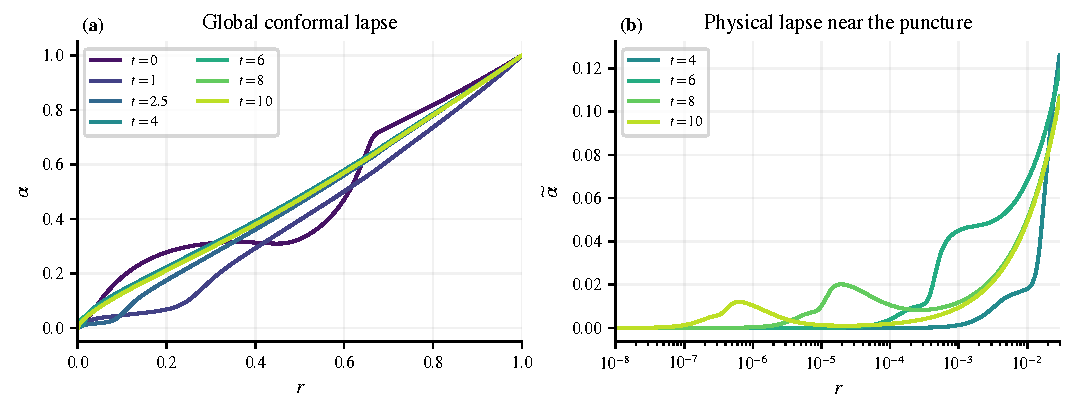
\includegraphics[width=\textwidth]{telegraph_lapse_evolution}
 \caption{Telegrapher lapse evolution on the finest completed grid, $N=4097$. The global panel uses conformal $\alpha$, which remains finite at scri. The inner panel uses physical $\widetilde\alpha=\alpha/\Omega$ and logarithmic radius to expose the late nonmonotone structure. Curves use saved profiles without smoothing or temporal interpolation. The remaining bump is not declared eliminated.}
 \label{fig:tele-lapse}
\end{figure*}
\begin{figure*}[tp]
 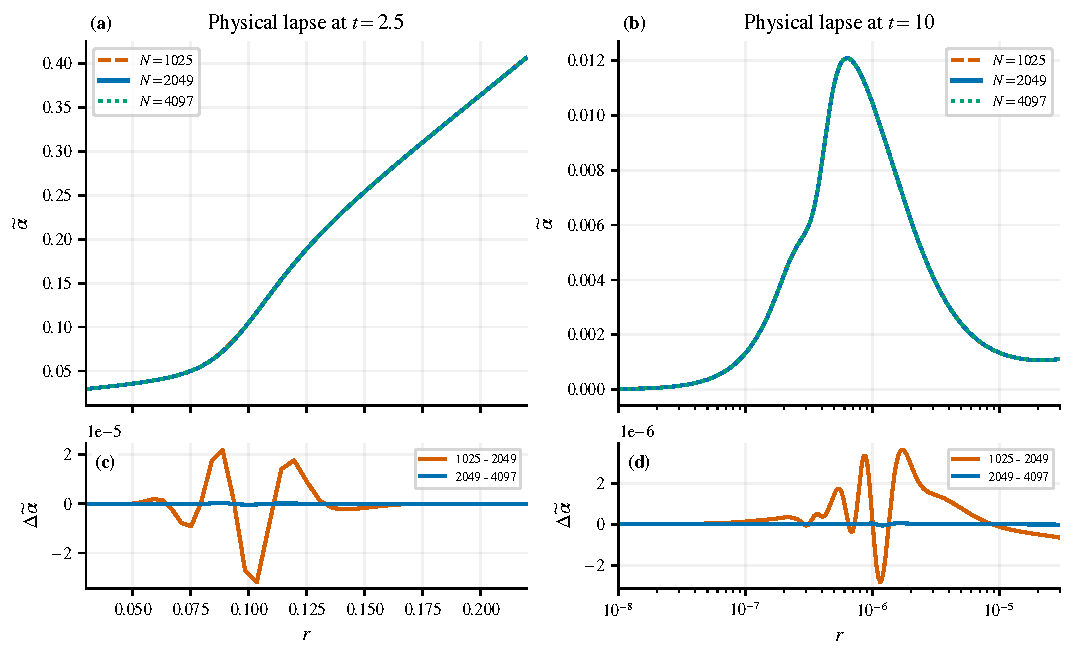
\includegraphics[width=\textwidth]{telegraph_lapse_resolution}
 \caption{Three-grid physical-lapse comparison at $t=2.5$ and $t=10$. The lower panels show raw consecutive-grid differences at matching physical nodes. The late panel retains the near-puncture structure instead of cutting it out. These are profile comparisons; whole-trajectory derivative and constraint checks are reported separately.}
 \label{fig:tele-resolution}
\end{figure*}

Figure~\ref{fig:tele-constraints} presents all four constraint histories. The radial RMS can be small while a sharply localized inner error is appreciable. At $t=10$ on $N=2049$, for example, $\normr{\HH}=9.67\times10^{-8}$ but $\max_r|\HH|=2.24\times10^{-3}$. That peak lies at $r=1.46\times10^{-6}$, well inside the apparent horizon at $r=0.10765$; the exterior maximum is $1.05\times10^{-7}$. This is a localization diagnostic, not an exterior-only acceptance rule. On the finest grid, the corresponding final full-grid maximum is \TeleFinalHMax\ at $r=\TeleFinalHRadius$, and the peak sampled apparent-horizon mass error over the full run is \TeleAHMassError. The maximum sampled finite-node Misner--Sharp mass discrepancy over the same trajectory is \TeleMSMassError, including the near-scri and inner nodes; the maximum sampled AF-end coefficient-mass discrepancy is \TeleAFMassError. The actual scri mass slot is undefined in this diagnostic and is not included in that finite-node maximum. Neither small exterior error nor accurate horizon mass overrides an inner constraint failure. Figure~\ref{fig:tele-inner} makes the pointwise error, growing lapse gradient, error location, and mass diagnostic visible together.

\begin{figure*}[tp]
 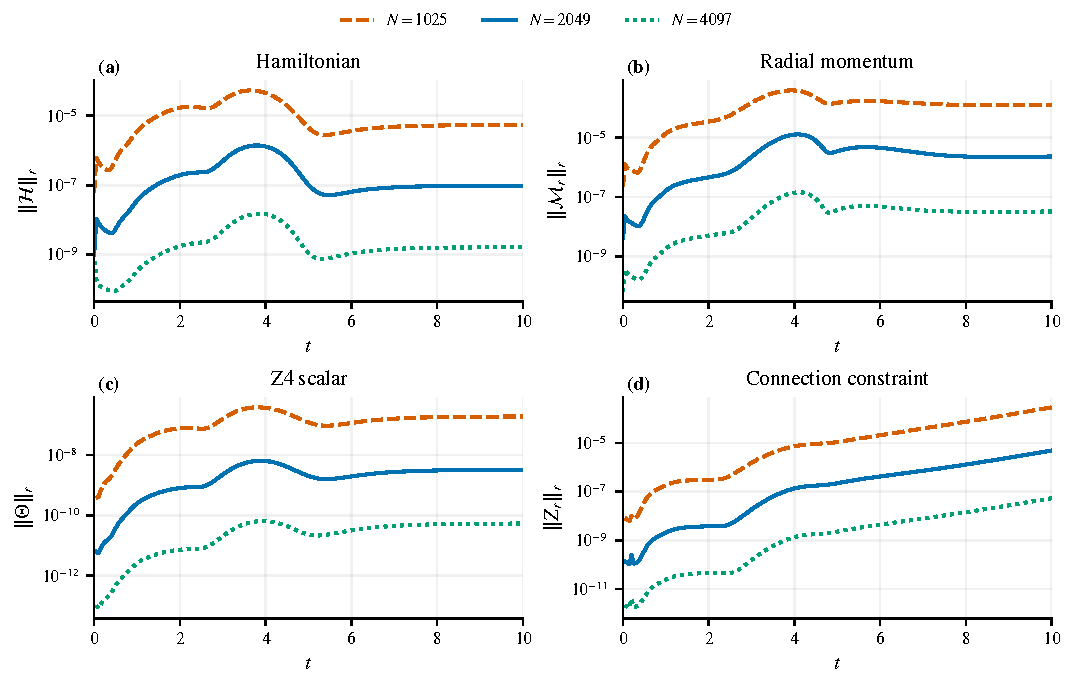
\includegraphics[width=\textwidth]{telegraph_constraints}
 \caption{Full-domain radial RMS constraints for the completed telegrapher sequence, using Eq.~\eqref{eq:telegraph-norm}. Every plotted value was recomputed from saved fields and checked against the recorded history. These curves sample every $0.05$ time units; the accepted-state maxima in Table~\ref{tab:telegraph} can be slightly larger. No interior mask is applied. The radial weighting suppresses small-radius contributions, so Fig.~\ref{fig:tele-inner} also reports the full-grid pointwise Hamiltonian error.}
 \label{fig:tele-constraints}
\end{figure*}
\begin{figure*}[tp]
 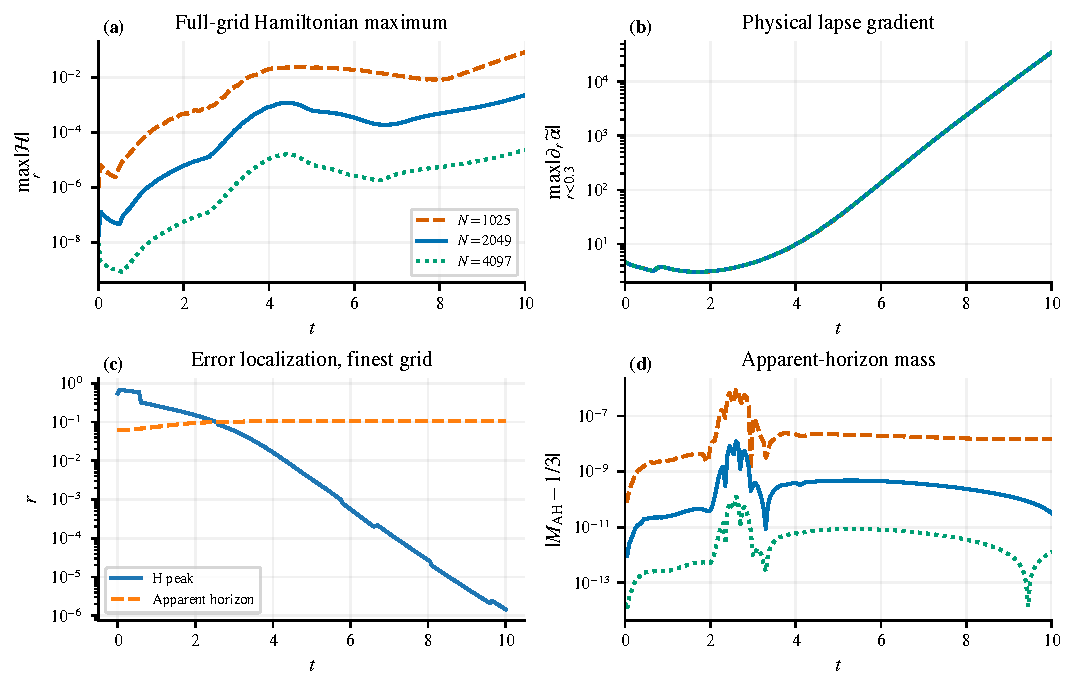
\includegraphics[width=\textwidth]{telegraph_inner_errors}
 \caption{Diagnostics that prevent a small radial RMS from hiding the inward layer. (a) Unweighted full-grid Hamiltonian maximum. (b) Physical-lapse gradient over $0\leq r<0.3$, evaluated with analytic AF factors and seven-point chart derivatives. (c) Position of the finest-grid Hamiltonian peak compared with the apparent horizon. (d) Independent apparent-horizon mass error. The horizon is identified from the outgoing expansion; this does not locate the event horizon. Mass errors near floating-point precision do not establish an asymptotic order.}
 \label{fig:tele-inner}
\end{figure*}

The tracked rays retain their ordering in the sampled spatial comparison. At $t=10$, all 81 inward rays remain active and all 81 outward rays have exited at scri. The finest minimum active inward $\log\mathcal J_-$ is \TeleMinLogJ, and the minimum active neighboring-ray separation is \TeleRayGap. The maximum middle-to-fine differences over the full trajectory are \TeleRayPositionError\ in ray position and \TeleRayLogError\ in $\log\mathcal J$, including terminal states. The observed peak-difference orders are \TeleRayPositionOrder\ and \TeleRayLogOrder, respectively. Figure~\ref{fig:tele-rays} shows the ray fans, compression, and refinement differences. These measurements describe strongly compressed finite-grid characteristics; they do not establish a continuum intersection or its absence.

\begin{figure*}[tp]
 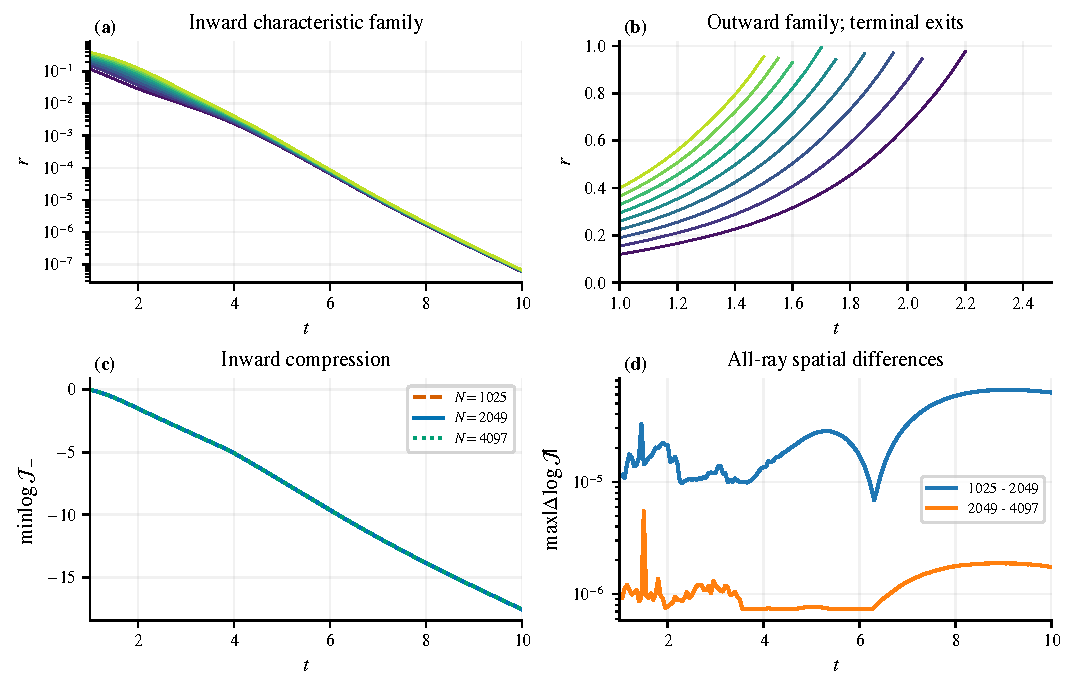
\includegraphics[width=\textwidth]{telegraph_characteristics}
 \caption{RK-stage characteristic tracking with matched dense exit events. The upper panels show nine representative seeds from each of the 81-ray families on $N=4097$. The outward panel zooms to the exit interval. Paths end at the last saved active point; no precise event time is fabricated from the plotting cadence. The lower-left panel shows inward compression across resolutions. The lower-right comparison includes all rays, including their frozen terminal compression. Positive finite-grid Jacobians and ordered rays are not a continuum shock-avoidance proof.}
 \label{fig:tele-rays}
\end{figure*}

\subsection{Independent timestep evidence at the stopping point}
The baseline and independent half-step $N=2049$ trajectories both reach $t=10$. The quarter-step control was paused at the requested finest-grid stopping point, with saved reports through $t=8.35$. Consequently the required full-duration three-level temporal-order and timestep-to-spatial-error assessment remains incomplete. The completed baseline--half-step comparison gives maximum bulk and endpoint field differences of $4.04\times10^{-12}$ and $2.33\times10^{-12}$, a Hamiltonian pointwise difference of $5.71\times10^{-10}$, and ray-position and $\log\mathcal J$ differences of $4.27\times10^{-13}$ and $7.68\times10^{-8}$. Two timestep levels alone do not establish temporal order. These raw differences, and the earlier short diagnostic pilot, cannot replace the missing robustness controls.



\subsection{Long-duration puncture pilot: exterior accuracy and termination}
\label{sec:tele-long}
A separate low-resolution continuation targeted $t=500$ on $N=1025$, starting from the verified $t=10$ checkpoint of the genuine wormhole trajectory. The frozen numerical source, binaries, map, CFL factor, relaxation parameters, and full-domain boundary treatment were unchanged. The run stopped at $t=43.836474609375$ with the native error \code{g=1 gauge or positivity violation}. Figure~\ref{fig:tele-long} reports all validated saved states through $t=43.8$, including the parent trajectory. The requested duration was not reached. This is a single-grid survival pilot, not an additional convergence study.

For this long-duration pilot we assess an apparent-horizon-exterior error budget and take apparent-horizon mass conservation as the primary invariant check. At each saved time, let $E(t)=\{i:r_i\geq r_{\rm AH}(t)\}$, where the existing outgoing-expansion finder locates $r_{\rm AH}$. With the same mapped radial weights $w_i=r_i^2(\dd r/\dd x)_i$ used previously, define
\begin{equation}
 \|C\|_{r,E}^2=\frac{\sum_{i\in E(t)}w_i C_i^2}{\sum_{i\in E(t)}w_i},
 \qquad C\in\{\HH,\MM,\Th,Z_r\}.
 \label{eq:exterior-norm}
\end{equation}
The pointwise budget uses $\max_{i\in E(t)}|C_i|$. Interior errors and puncture-end mass estimates are excluded from this budget. The normalization uses only exterior weights, rather than filling the excluded interior with zeros. This is a diagnostic selection: the evolution still includes every puncture-interior node. The historical three-grid full-domain assessment through $t=10$ remains unchanged and is labeled separately.

At the last saved time $t=43.8$, the exterior RMS values for $(\HH,\MM,\Th,Z_r)$ are $(1.79\times10^{-7},2.44\times10^{-6},5.00\times10^{-8},5.21\times10^{-7})$. The exterior Hamiltonian maximum is $5.88\times10^{-6}$. These late values remain nearly unchanged from $t=10$. The initial transient remains in the budget: the maximum sampled exterior Hamiltonian and momentum RMS values on $0\leq t\leq43.8$ are $1.84\times10^{-5}$ and $4.92\times10^{-5}$. The apparent-horizon mass error is $3.93\times10^{-8}$ at $t=43.8$, or $1.18\times10^{-7}$ relative to $M=1/3$; its peak sampled absolute error over the whole interval is $8.79\times10^{-7}$, corresponding to relative error $2.64\times10^{-6}$. The late mass error grows gradually while remaining below the initial-transient peak.

The saved exterior diagnostics do not show a blow-up before termination. Nevertheless, excluding interior diagnostic errors does not disable the full-domain evolution guard. The termination checkpoint remains finite, its metric deviation is exactly zero, and reconstructed lapse and conformal factor are positive at positive-radius nodes. The generic guard message does not preserve the offending stage or radial index. An offline replay, described below, localizes the failure to lapse underflow at the second positive-radius node during RK stage four. Puncture-interior constraints and mass estimates remain archived diagnostics and are excluded from the exterior budget. The result supports preserved horizon mass and a nearly steady late exterior constraint budget through the last saved profile, but does not establish survival to $t=500$ or exterior convergence. The failed trajectory is retained; the following floor controls are separate experiments.

\begin{figure*}[tp]
 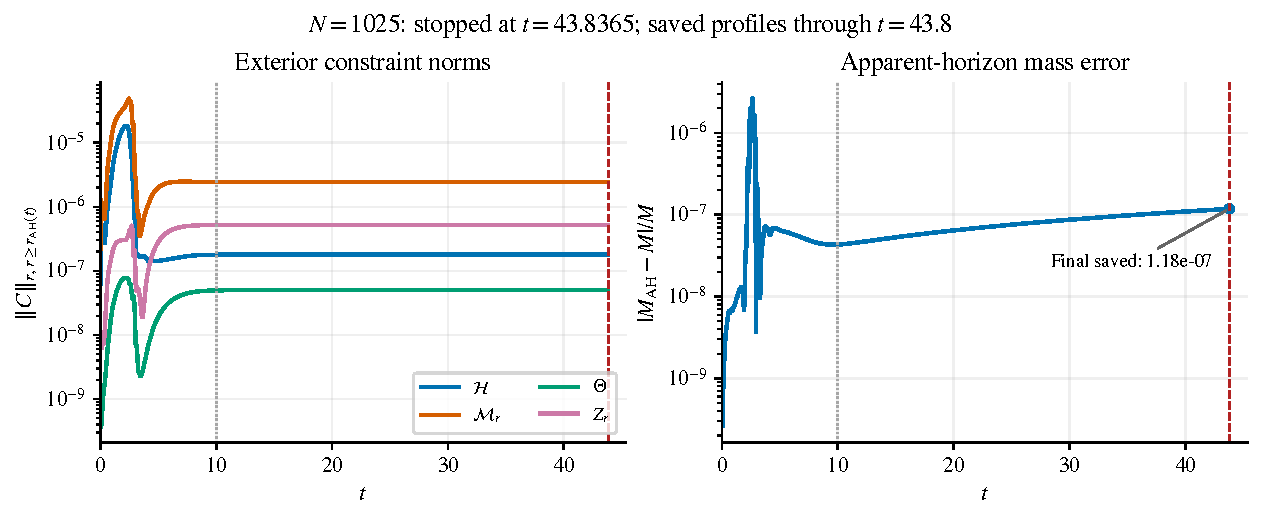
\includegraphics[width=\textwidth]{telegraph_long_exterior_status}
 \caption{Final saved history of the $N=1025$ puncture continuation targeting $t=500$. Left: apparent-horizon-exterior radial RMS constraints, normalized over the exterior region at each saved time. Right: relative apparent-horizon mass error, the primary invariant in the revised long-run budget. The gray dotted line marks the verified restart at $t=10$; the red dashed line marks the native guard stop at $t=43.8365$. Curves end at the last saved time $t=43.8$ and are not extrapolated to the failed stage. Puncture-interior errors and puncture mass estimates do not enter this budget. All 877 distinct saved profiles were checked for finite fields, reconstructed full-domain norms, and independently recomputed apparent horizons before evaluating the exterior diagnostics.}
 \label{fig:tele-long}
\end{figure*}


\subsection{Localized lapse underflow and a configurable floor}
\label{sec:lapse-floor}
Replaying the failed step on an isolated checkpoint copy with its frozen kernels reproduces the native rejection without advancing the original trajectory. At the second positive-radius node, $r=3.63\times10^{-9}$, the conformal lapse falls from $5.20\times10^{-11}$ at stage one to $1.25\times10^{-11}$ and $1.37\times10^{-13}$ at stages two and three. The fourth-stage value has $\log\alpha=-1109.3$, so reconstruction underflows to zero. The metric deviation remains zero and the conformal factor remains positive. The telegrapher contribution to the logarithmic lapse rate is approximately $-5.87\times10^4$, $-2.44\times10^5$, and $-2.22\times10^7$ in the first three stages, whereas the base-gauge contribution is positive and only of order $10^2$. Thus the additive flux contribution divided by the collapsing lapse drives the immediate rejection. Figure~\ref{fig:lapse-stop} shows the increasingly irregular inner profile and the replayed stage values.

We added the user-configurable input \code{lapse_floor}, with default $10^{-10}$ and $0$ to disable it. The CLI spelling is \code{--lapse-floor}. At ordinary nodes $0<r<1$, the numerical update applies
\begin{equation}
 \widetilde\alpha_i\leftarrow\max(\widetilde\alpha_i,\alpha_{\min}),
 \qquad \alpha_{\min}=10^{-10}\quad\hbox{by default},
\end{equation}
before each RK stage and after every accepted step, including initialization before the first report. The projection is implemented in the logarithmic lapse chart with an upward rounding margin. Only the clipped accepted lapse components have their compensated-update remainder reset. The AF coefficient endpoint and scri clock are unchanged; no constraint or other geometric field is projected. This is a finite-grid regularization of the unresolved interior, not an established continuum AF-end prescription. Historical inputs are explicitly pinned to zero floor, and the selected value is included in restart validation.

The native implementation with zero floor still reproduces the original rejection. With $\alpha_{\min}=10^{-10}$, a separate checkpoint control completes 20\,480 steps, one additional time unit, to $t=44.8365$. Only the first two positive-radius nodes require clipping in this control. Its final relative apparent-horizon mass error is $1.20\times10^{-7}$ and its exterior Hamiltonian RMS is $1.79\times10^{-7}$. Preliminary isolated controls with floors $10^{-8}$ and $10^{-6}$ also complete one time unit; these short controls do not establish long-duration stability. Seven targeted telegrapher test groups pass, including independent projected-RK comparison, preserved endpoint slots, disabled and invalid inputs, and exact floor-bound checkpoint restart. A separate fresh $N=1025$ wormhole trial with the default floor also targeted $t=500$. Its terminal outcome is reported below, separately from the unfloored failure and the completed three-grid study.

\begin{figure*}[tp]
 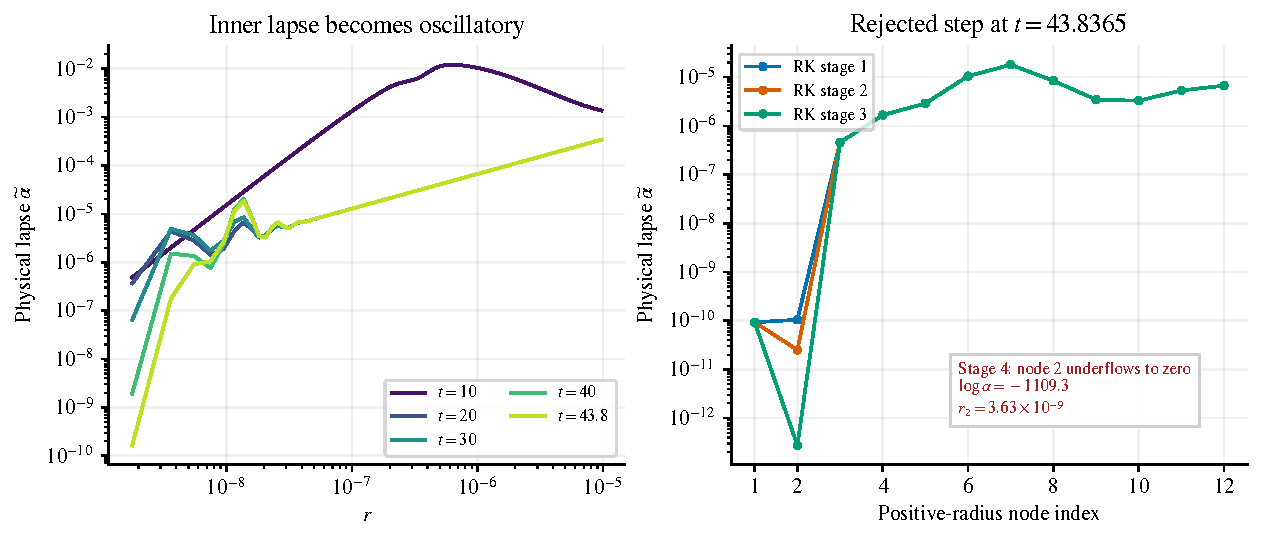
\includegraphics[width=\textwidth]{telegraph_lapse_stop}
 \caption{Diagnosis of the unfloored termination. Left: raw physical-lapse profiles in the innermost resolved region, showing irregular structure concentrated near the first few grid points. Right: the first three stages of an offline replay of the rejected step, using the frozen original kernels. Node two reaches $\log\alpha=-1109.3$ at stage four and underflows to zero; that zero is stated rather than plotted on the logarithmic axis. This local failure occurs far inside the apparent horizon. The floor controls are separate numerical experiments and do not overwrite this evidence.}
 \label{fig:lapse-stop}
\end{figure*}


\subsection{Terminal outcome of the floored duration trial}
\label{sec:floored-long}
The fresh wormhole trial with $\alpha_{\min}=10^{-10}$ stops at $t=84.798291015625$, after 1\,736\,669 accepted steps, with the native error \code{telegraph coupled-speed/relaxation timestep guard}. All 1696 saved profiles through $t=84.75$ were validated with the same source-binding, field-finiteness, full-domain-norm, and independent horizon checks used for the unfloored export. The original failed trajectory is preserved; this trial begins at $t=0$ with the floor applied to the analytic pre-collapsed lapse.

Figure~\ref{fig:floored-long} separates the exterior budget from the unresolved inner behavior. At $t=84.75$, the exterior RMS values for $(\HH,\MM,\Th,Z_r)$ are $(1.79\times10^{-7},2.44\times10^{-6},5.00\times10^{-8},5.21\times10^{-7})$, nearly unchanged from their late unfloored values. The exterior Hamiltonian maximum is $5.88\times10^{-6}$. The final saved apparent-horizon mass error is $7.01\times10^{-8}$, or $2.10\times10^{-7}$ relative to $M=1/3$. The maximum sampled relative error, $2.64\times10^{-6}$, still occurs during the initial transient. The last saved scri pole residue is $4.59\times10^{-13}$, with zero clock and nullness residuals. These statements apply to saved states, not to a successful continuation through the rejected step.

The floor remains localized far inside the apparent horizon: its outermost activation over the trajectory is $r=6.29\times10^{-7}$, compared with $r_{\rm AH}\simeq0.10765$. Nevertheless, the maximum upward correction to the stored lapse logarithm grows to $5.25\times10^3$ by the last saved state and $1.20\times10^4$ in the terminal diagnostics. This is substantial numerical clipping, rather than a uniformly small perturbation. The lower bound prevents lapse underflow but does not bound the independently evolved geometry or the elliptic shift.

An isolated replay with the exact frozen kernels reproduces the guard at the first stage of the next attempted step. The maximum occurs at positive-radius node three, $r=5.53\times10^{-9}$, where the physical lapse remains $10^{-10}$ but the reconstructed shift is $\beta^r\simeq3.93\times10^7$. Both coupled characteristic speeds are approximately $-3.93\times10^7$: shift transport dominates their splitting. With the mapped Jacobian $\dd r/\dd x=1.98\times10^{-6}$ and $\Delta t=4.8828125\times10^{-5}$, the checked mapped Courant number is $9.94\times10^{11}$, exceeding the limit $0.4$. The relaxation ratio remains $\Delta t/\tau=0.0024414$, so the speed condition triggers this guard. The last saved accumulated Courant maximum was only $0.2000$; the terminal event is not inferred by extrapolating that sampled history. The replay changes neither parameters nor timestep and does not continue the failed trajectory. Subsequent fresh repair trials are assessed separately in Sec.~\ref{sec:tele-repair-evidence}. The evidence establishes a later discrete inner failure despite a preserved saved exterior budget, not survival to $t=500$, continuum shock formation, or convergence of the floor prescription.

\begin{figure*}[tp]
 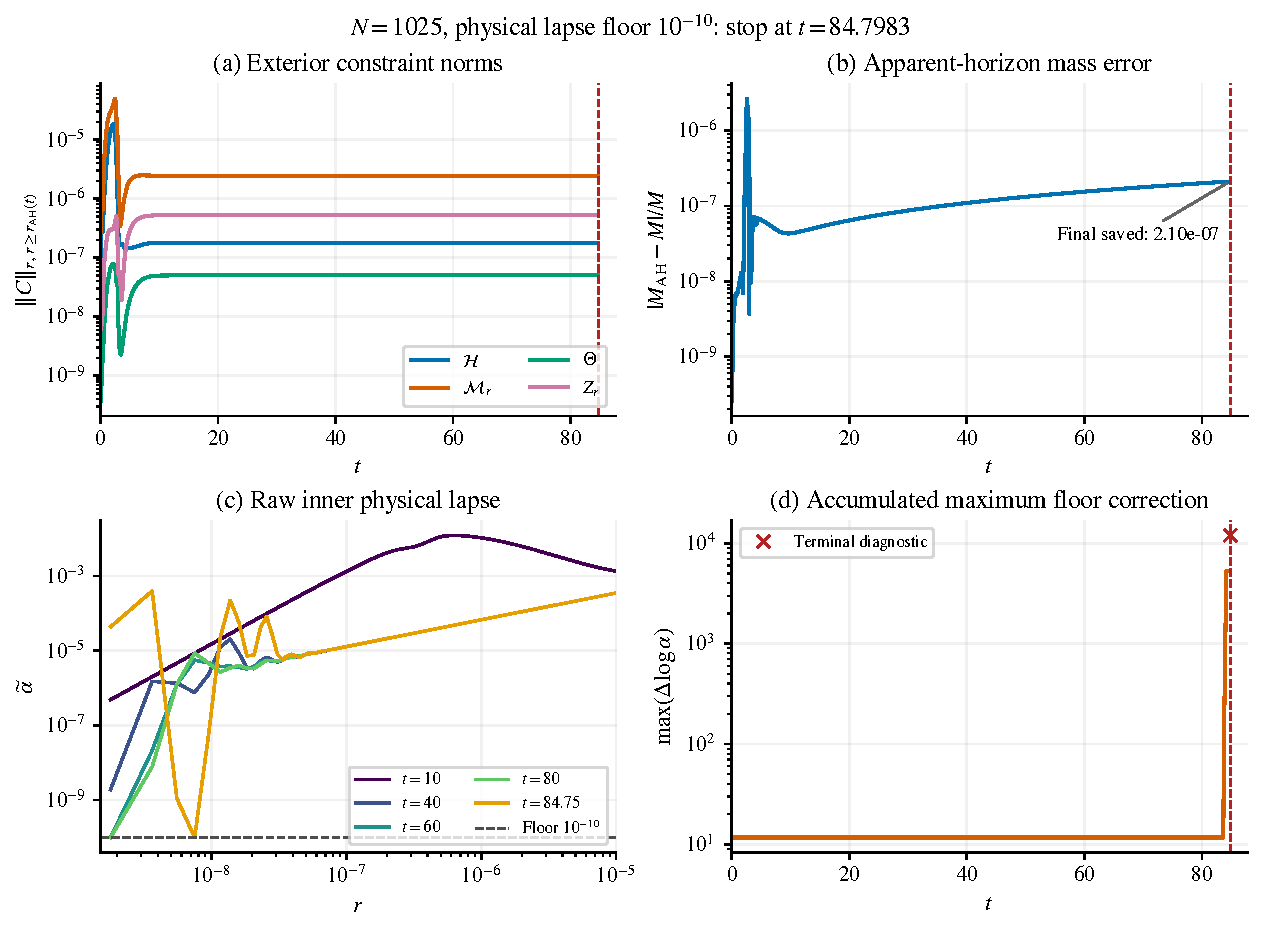
\includegraphics[width=\textwidth]{telegraph_floored_long}
 \caption{Separate fresh wormhole trial with physical lapse floor $10^{-10}$. (a) Apparent-horizon-exterior RMS constraints. (b) Relative apparent-horizon mass error. These primary diagnostics retain the complete initial transient and exclude the horizon interior. (c) Raw inner physical-lapse profiles, with the imposed floor marked; no smoothing is applied. (d) Accumulated maximum upward correction to the stored lapse logarithm, with the terminal diagnostic marked separately from the saved histories. The vertical red lines mark the speed-guard stop at $t=84.7983$; saved histories end at $t=84.75$. Large interior clipping is disclosed but is not substituted for the requested exterior error budget.}
 \label{fig:floored-long}
\end{figure*}
